\documentclass[11pt]{article}
\usepackage[a4paper,total={160mm,250mm}]{geometry}
\usepackage{amssymb}
\usepackage{amsmath}
\usepackage[ruled,linesnumbered]{algorithm2e}
\usepackage{hyperref}
\usepackage{cleveref}
\usepackage{listings}
\usepackage{indentfirst}
\usepackage{tikz}
\usepackage{pgfplots}
\usetikzlibrary{arrows.meta}
\usepackage{listings}

\SetKwComment{Comment}{/* }{ */}

\lstdefinestyle{main}{
    keywordstyle=\color{magenta},
    numberstyle=\tiny\color{codegray},
    stringstyle=\color{codepurple},
    basicstyle=\ttfamily\footnotesize,
    captionpos=b,
    keepspaces=true,
    numbersep=5pt,
    showspaces=false,
    showstringspaces=false,
    showtabs=false,
    tabsize=2
}


\lstset{style=main}

\author{Rosie Bartlett\\\texttt{lvff38@durham.ac.uk}}
\title{Clique number in polynomial time}

\begin{document}
\maketitle

\abstract{
In this paper I will present the neighbourhood group algorithm for finding $\omega(G)$ in $O(n^4)$ time using node neighbourhoods and grouping.
}

\section{The problem}
The problem is henceforth defied as follows; for any arbitrary graph with $n$ nodes, find the size of the largest clique, that is a subgraph for which any node is adjacent to any other node in that subgraph.

\section{Algorithm}
Please note here that the traditional $G=(V,E)$ has been replaced with a set for $V$. this is to simplify algorithm notation. I also define $N(n)\forall n\in V$ as the set of nodes adjacent to $n$ and not the induced subgraph.
\begin{algorithm}
\caption{Clique number calulation}\label{alg:main}
\KwData{$G=(V,E)$}
\KwResult{$\omega(G)$}
$k\gets 0$\\
\ForEach{$n_1\in V$}{
	\eIf{$N(n_1)=\emptyset$}{
		$k\gets\max\{k,1\}$\\
	}{
		\If{$|N(n_1)|\geq k$}{
			\ForEach{$n_2\in N(n_i)$}{
				$I\gets N(n_1)\cap N(n_2)$\\
				$t\gets 0$\\
				\While{$I\neq\emptyset$}{
					select $n_3$ from $I$\\
					$t\gets\max\{t,|I\cap N(n_3)| + 1\}$\\
					$I\gets I\setminus N(n_3)$
				}
				$k\gets\max\{k,t+2\}$\\
			}
		}
	}
}
\Return{$k$}
\end{algorithm}

This algorithm can be considered to take all possible pairs of adjacent nodes and find their cliques. To find the cliques containing the two given nodes, we group the intersection of their neighbourhoods. If we consider \cref{fig:groups}, we have three maximal cliques made of $n_1$ and $n_2$ along with the groups $\{m_1,m_2,m_3\}$, $\{p_1,p_2\}$, and $\{p_3\}$. We can be sure that these are the only cliques that contain $n_1$ and $n_2$ otherwise there would be more nodes in $I$ represented as the row of nodes.

\begin{figure}[h]
	\centering
	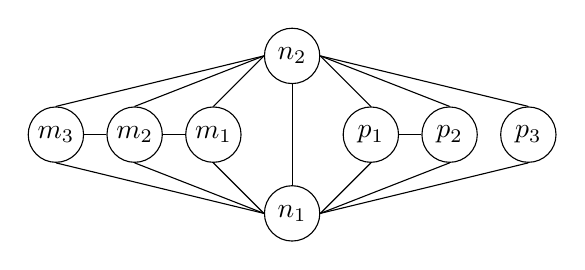
\begin{tikzpicture}[shorten >=1pt,->]
		\tikzstyle{node}=[circle,minimum size=20pt,inner sep=2pt,draw=black]
		\node[node] (n1) at (0,0) {$n_1$};
		\node[node] (n2) at (0,2) {$n_2$};
		\draw (n1) -- (n2) -- cycle;
		\foreach \x in {1,...,3}{
			\node[node] (p\x) at (\x,1){$p_\x$};
			\draw (n1.east) -- (p\x.south) -- cycle;
			\draw (n2.east) -- (p\x.north) -- cycle;
			
			\node[node] (m\x) at (-\x,1){$m_\x$};
			\draw (n1.west) -- (m\x.south) -- cycle;
			\draw (n2.west) -- (m\x.north) -- cycle;
		};
		\draw (p1) -- (p2) -- cycle;
		\draw (m1) -- (m2) -- (m3) -- cycle;
	\end{tikzpicture}
	\caption{Conceptualisation of grouping $N(n_1)\cap N(n_2)$}
	\label{fig:groups}
\end{figure}

\subsection{Time complexity}

To analyse the time complexity of \cref{alg:main}, I will consider sections of the algorithm for a graph $G$ with $n$ nodes.\\

Firstly, the main loop (lines 2-17) runs $n$ times. We then reach a conditional which we will assume the else condition (lines 5-16) since it has the larger time complexity and will give the worst case complexity for the algorithm. We then reach a second conditional (lines 6-15). This is here for optimisation. We will assume that this runs for each node for the worst case. The loop inside this condition (lines 7-14) runs at most $n-1$ times when the current node is connected to all other nodes. The while loop (lines 8-13) will run up to $n-2$ times in the case that $n_1$ and $n_2$ are connected to all the other nodes, each of which are connected to only $n_1$ and $n_2$. The section within the while loop (lines 10-12) will run in linear time since al operations can be performed within linear time by use of fixed length arrays for set operations.

We also precompute $N(n)\forall n\in V$ taking at most $O(n^3)$\footnote{$n$ repetitions of going through each edge for which there are at most $\frac{n(n-1)}{2}$ giving $O(n^3)$}.

In total this gives $O(n^3)+O(n^4)=O(n^4)$ for the algorithm.

\subsection{Lower bound}
This algorithm has a lower bound of $\Omega(1)$ for a graph with one node. This is not very useful, so we instead consider the best case performance for a graph with $n$ nodes.\\

In this graph, we would find the largest clique in the first iteration which would contain all the nodes in the graph giving the largest possible $k$ value of $n$. This means that the first iteration would take linear time by the set operations. Any following iteration would take constant time since very little is actually run giving a total of $\Omega(n)$ for the lower bound. This is excluding the neighbourhood pre-computation.

\section{Correctness}

Let $n_1$ be a node in $V$. If we consider the possible cliques $n$ is contained within, by definition all of these cliques must contain nodes within $N(n_1)$ otherwise $n$ would not be adjacent to all nodes in the subgraph, and thus the subgraph would not be a clique. We now place a condition on the following section. If $|N(n_1)|$ is less than the size of the current largest clique, there is no possible way in which this node will give a larger clique and we can ignore it. If this is not the case we continue. By then taking $n_2\in N(n_1)$, any clique that $n_2$ is contained within must contain nodes within $N(n_2)$ for the same reason. Therefore, any clique that contains both $n$ and $n_2$ can only contain nodes within $N(n_1)$ and $N(n_1)$ or $N(n_1)\cap N(n_2)$ which we will call $I$.

It is not guaranteed that $I$, along with $n_1$ and $n_2$, will be a clique however since nothing we have done thus far would allow us to assume this without loss of generality. We can assume though that any two unique nodes in $I$ there is a path between them with a length of 2 through either $n_1$ or $n_2$. If we then go through each $n_3\in I$ and take $\{n_1,n_2\}\cup (I\cap N(n_3))$ we end up with a clique since each node in $I$ is at adjacent to both $n_1$ and $n_2$, and each node in $N(n_3)$ is adjacent to $n_3$ which means that each node in $I\cap N(n_3)$ is adjacent to $n_1$, $n_2$, $n_3$. This is an improvement since in $I$ there were nodes that were 2 away, but by constraining $I$ by the neighbourhood of a node in $I$ we remove any nodes in $I$ that are not adjacent to the currently considered node in $I$ giving a clique.

Unlike when working through $N(n_1)$, we can filter out some of the nodes in $I$ as we go to increase speed since we're not considering the entirety of $N(n_3)$, but only finding connected sections in $I$.

This does not find all the cliques in the graph. It does however find the largest cliques given two adjacent nodes which allows us to then give $\omega(G)$ which would them allow us to state the existence of a $k$-clique in $G$.

\section{Conclusion}

This paper has presented a polynomial time algorithm for finding all cliques for an arbitrary undirected graph. There is room for improvement in the given algorithm. For example one might improve the number of iterations by not computing identical cliques; for example in $C_3$ each iteration, two nodes in $N(n)$ are considered, each functionally equivalent, and then the process repeats three times for equally functionally equivalent nodes. These optimisations, other than those given, are left for future research.

\appendix
\section{Python implementation}
Here a graph is represented as a dictionary with each key value pair being a node, the key being the node index, and the value being the nodes connected to the current node.
\lstinputlisting[language=Python,caption={Neighbourhood search algorithm for finding the maximal clique in a graph in $O(n^4)$ time. Written in Python 3.x}]{main.py}
\end{document}
